\section{1174079 - Chandra Kirana Poetra}
Chapter 2 - Membangun model prediksi
\subsection{Teori}
\subsubsection{Jelaskan Apa Itu Binary Classification dilengkapi ilustrasi gambar sendiri.}
\hfill\\
\begin{figure}[H]
    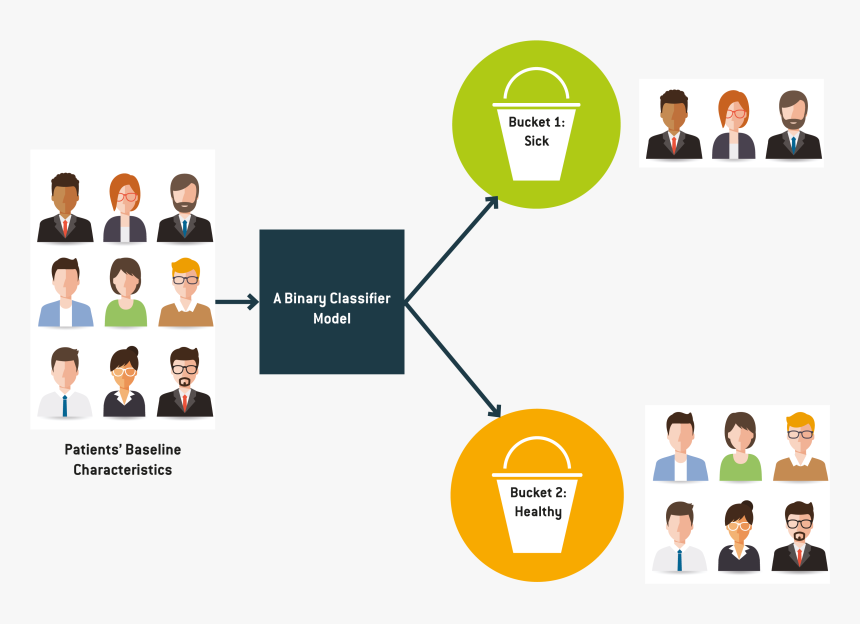
\includegraphics[width=12cm]{figures/1174079/2/binaryclassification.png}
    \centering
    \caption{Ilustrasi Binary Classification}
\end{figure}

Klasifikasi biner merupakan suatu cara kerja atau metode dalam menentukan atau mengelompokkan beberapa elemen atau data menjadi dua kelompok (Menentukan klasifikasi tiap data yang ada) berdasarkan aturan klasifikasi. Konteks yang membutuhkan suatu keputusan mengenai apakah suatu data atau item memiliki sifat kualitatif atau tidak, beberapa karakteristik tertentu yang unik,atau beberapa klasifikasi biner yang tipikal meliputi:
\begin{itemize}
	\item Tes medis : digunakan untuk menentukan apakah seorang pasien memiliki penyakit tertentu atau tidak, bentuk klasifikasinya disini yaitu keberadaan penyakitnya itu sendiri
	\item Suatu metode "pass or fail" yang menentukan suatu spesifikasi apakah sudah memenuhi ketentuan atau belum.
	\item Pengambilan informasi : Menentukan apakah suatu halaman atau artikel berhak untuk tampil dalam suatu result set dari hasil pencarian atau tidak, properti klasifikasi disini adalah relevansi artikelnya itu sendiri atau kegunaannya kepada para pembaca..
\end{itemize}

\subsubsection{Jelaskan Apa itu supervised learning , unsupervised learning dan clusterring dengan ilustrasi gambar sendiri.}
\begin{enumerate}
\item supervised learning
\hfill\\
Supervised learning merupakan suatu metode dalam bidang machine learning yang digunakan untuk melatih mesin menggunakan data yang sudah dilabeli. itu berarti beberapa data sudah dilabeli sebagai jawaban yang benar atau true. ini semua sama halnya seperti bagaimana seorang guru mengajarkan ilmu kepada para siswanya.

Algorithma Supervised learning belajar dari data training yang sudah dilabeli, yang kemudian akan membantu anda dalam memprediksi hasil yang akan terjadi dari data yang ada.
\begin{figure}[H]
    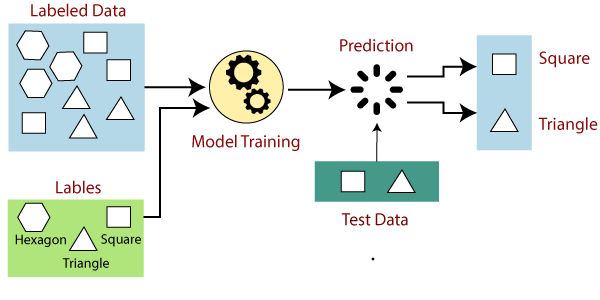
\includegraphics[width=12cm]{figures/1174079/2/supervisedmachinelearning.png}
    \centering
    \caption{Illustrasi cara kerja Supervised Learning}
\end{figure}

\item unspervised learning
\hfill\\
Unsupervised learning merupakan suatu algoritma di machine learning yang digunakan untuk menarik kesimpulan dari suatu dataset yang berisi data yang akan dinput tetapi tidak memiliki label.

Metode yang sering dipakai dalam Unsupervised learning  adalah analisis cluster, yang menggunakan data untuk menganalisis beberapa pola yang terlihat untuk mengelompokan suatu data. Data akan dikelompokan berdasarkan kemiripan dengan menggunakan basis seperti misalkan Euclidean atau proabilistic distance 
\begin{figure}[H]
    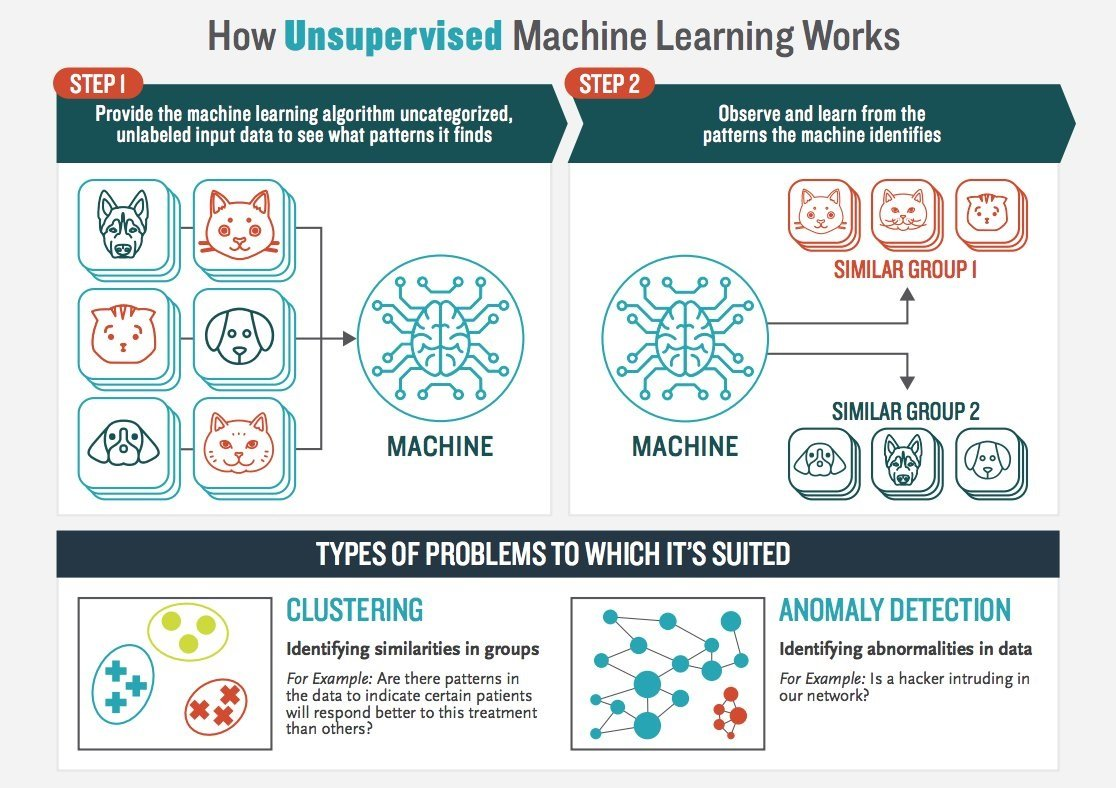
\includegraphics[width=12cm]{figures/1174079/2/unsupervisedmachinelearning.jpg}
    \centering
    \caption{Illustrasi cara kerja unsupervised learning}
\end{figure}

\item Clustering 
\hfill\\
\begin{figure}
Clustering adalah suatu proses untuk mengelompokkan entity yang mirip secara bersamaan, tujuan dari metode Clustering yang merupakan bagian dari Unsupervised machine learning sendiri adalah untuk mencair kemiripan dari data data yang ada.
    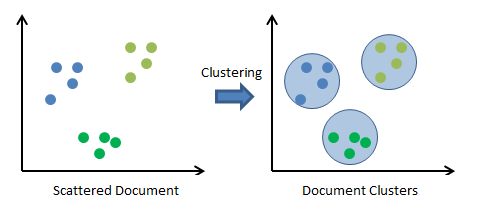
\includegraphics[width=12cm]{figures/1174079/2/clustering.png}
    \centering
    \caption{gambaran clustering}
\end{figure}
\end{enumerate}
\subsubsection{Jelaskan apa itu evaluasi dan akurasi dan disertai ilustrasi contoh dengan gambar sendiri}
\hfill\\
Evaluasi merupakan tahap untuk mengidentifikasi seberapa baik hasil dari suatu proses yang bekerja untuk kemudian ditingkatkan atau diperbaiki kembali agar mendapatkan hasil yang meningkat atau hasil yang ingin kita dapatkan.Sedangkan akurasi sendiri yaitu mengukur bagaimana suatu klasifikasi membuat keputusan yang benar. Di machine learning sendiri, kita bisa mengevaluasi kinerja dari machine learning itu dengan menggunakan hal yang disebut sebagai confusion matrix 
\begin{figure}[H]
    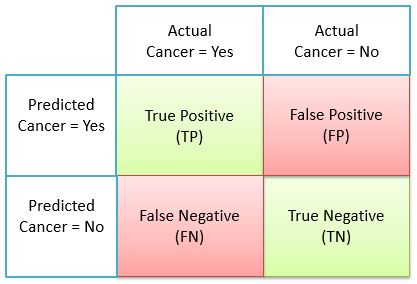
\includegraphics[width=12cm]{figures/1174079/2/confusionmatrix.jpg}
    \centering
    \caption{contoh confusion matrix}
\end{figure}

\subsubsection{Jelaskan bagaimana cara membuat Confusion Matrix, Buat confusion matrix sendiri.}
\hfill\\
\begin{enumerate}
    \item Pertama, kita harus punya dataset sebagai contoh, satu kolom untuk hasil yang diinginkan, dan satu kolum untuk contoh hasil prediksi machine learning
\begin{figure}[H]
    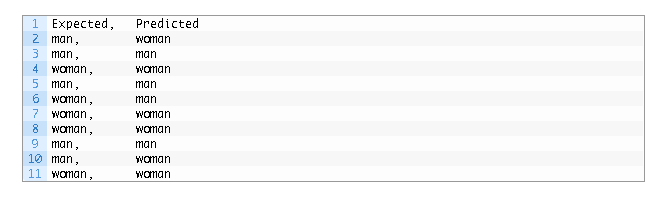
\includegraphics[width=12cm]{figures/1174079/2/confusionmatrixcara1.PNG}
    \centering
    \caption{Tahap 1 Confusion matrix}
\end{figure}	
    \item Kemudian kita translate koding tersebut menjadi python seperti berikut
\begin{figure}[H]
    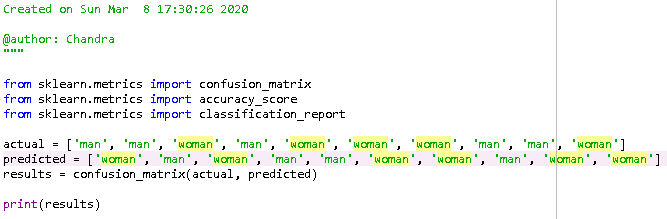
\includegraphics[width=12cm]{figures/1174079/2/confusionmatrixcara2.PNG}
    \centering
    \caption{Tahap 2 confusion matrix}
\end{figure}	
    \item Jalankan, dan lihat hasilnya
\begin{figure}[H]
    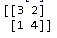
\includegraphics[width=12cm]{figures/1174079/2/confusionmatrixcara3.PNG}
    \centering
    \caption{Tahap 3 confusion matrix}
\end{figure}	
    \item Hasilnya, lelaki yang teridentifikasi sebagai lelaki adalah 3 orang, lelaki yang teridentifikasi sebagai perempuan sebanyak 2 orang, perempuan yang teridentifikasi sebagai lelaki sebanyak 1 orang dan perempuan yang teridentifikasi sebagai perempuan ada sebanyak 4 orang
    \item rumus prediksi adalah sebagai berikut 
\begin{figure}[H]
    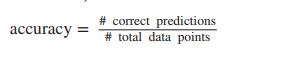
\includegraphics[width=12cm]{figures/1174079/2/confusionmatrixcara4.PNG}
    \centering
    \caption{Tahap 4 confusion matrix}
   \item Menggunakan rumus diatas, berarti jumlah akurasi yang didapat yaitu akurasi = total prediksi / jumlah data. yang berarti akurasi = 7 / 10 = 0,7 atau 70 \%
\end{figure}	
\end{enumerate}

\subsubsection{Jelaskan bagaimana K-fold cross validation bekerja dengan gambar ilustrasi contoh buatan sendiri.}
\hfill\\
Cara kerja k-fold validation adalah dengan cara membagi sample data secara acak sejumlah k yang kita definisikan sebagai jumlah subsample. Misalkan kita punya 12 data, dan kita definisikan k = 3, berarti kita akan membagi jumlah data 12 itu menjadi 3 bagian yang berisi masing masing 4 data, kemudian bagian 1 ini akan kita jadikan sebagai data yang akan digunakan untuk validasi, dan sisanya yaitu bagian 2 dan 3 menjadi training data, setelah itu data pada bagian 1 akan digunakan untuk memvalidasi data pada bagian 2 dan 3 yang kemudian apabila bagian satu sudah selesai dijadikan sebagai validasi data, maka tahap selanjutnya yaitu data pada bagian 2 akan dijadikan data untuk memvalidasi data pada bagian 1 dan 3, dan begitu seterusnya.
\begin{figure}[H]
    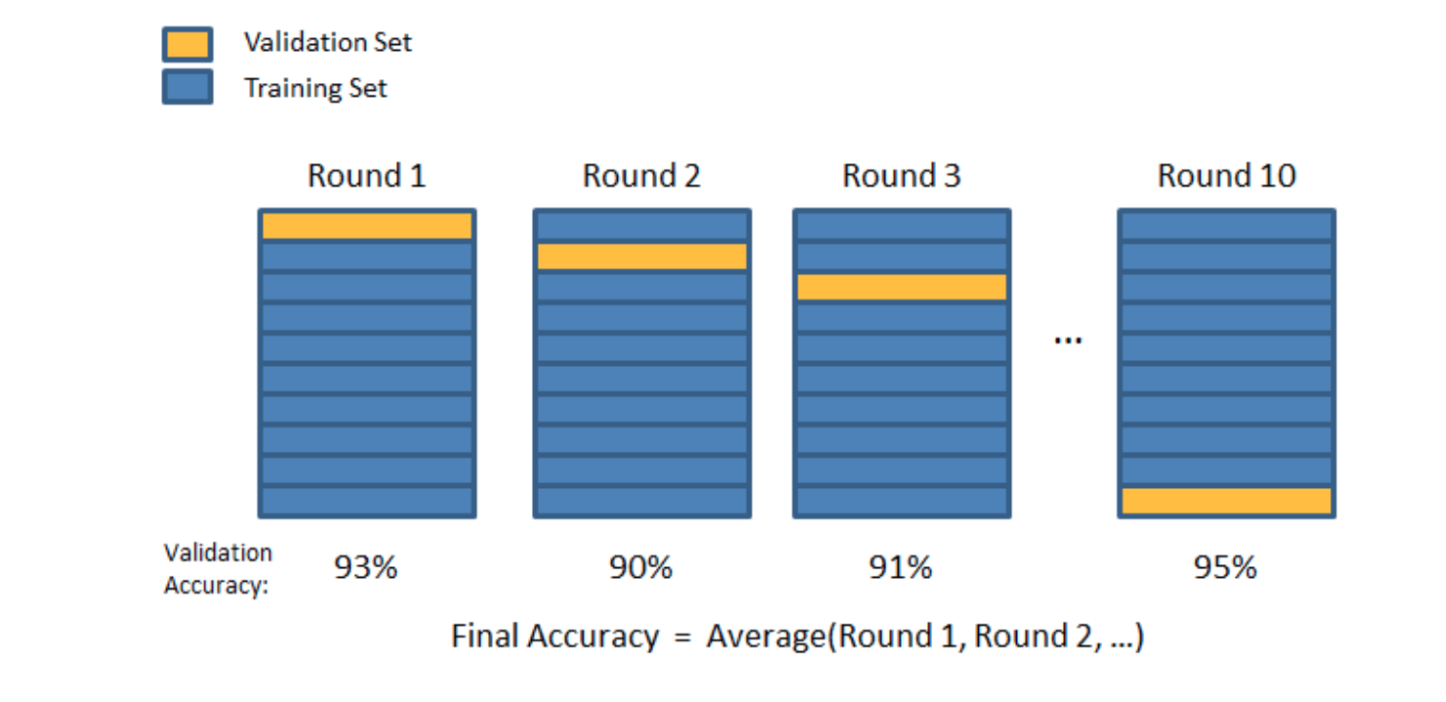
\includegraphics[width=8cm]{figures/1174079/2/kfold.PNG}
    \centering
    \caption{contoh K-Fold Validation}
\end{figure}

\subsubsection{Jelaskan Apa itu decision tree dengan gambar ilustrasi contoh buatan sendiri.}
\hfill\\
Decision Tree merupakan suatu konsep untuk yang berisi aturan aturan keputusan. Manfaat dari decision tree sendiri adalah untuk mempermudah pengambilan keputusan yang rumit menjadi lebih sederhana dan tergambarkan sehingga nantinya akan lebih mudah dalam proses pengambilan keputusan.
\begin{figure}[H]
    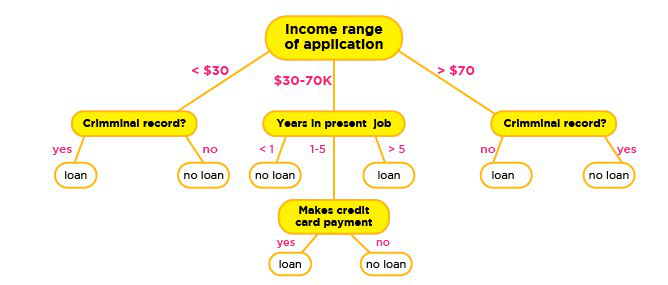
\includegraphics[width=8cm]{figures/1174079/2/decisiontree.png}
    \centering
    \caption{Decision Tree bermain Credit}
\end{figure}


\subsubsection{jelaskan apa itu information gain dan entropi dengan gambar ilustrasi buatan sendiri.}
\hfill\\
\begin{enumerate}
	\item information Gain
	\hfill\\
	Information gain merupakan cara untuk memberi nilai pada suatu informasi dengan cara rumus dibawah ini
\begin{figure}[H]
    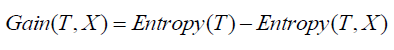
\includegraphics[width=12cm]{figures/1174079/2/informationgainrumus.PNG}
    \centering
    \caption{information gain}
\end{figure}

	\item Entropi
	\hfill\\
	Entropi adalah nilai informasi yang menyatakan ukuran ketidakpastian(impurity) dari attribut dari suatu kumpulan obyek data dalam satuan bit. Lihat gambar sebagai ilustrasi
\begin{figure}[H]
    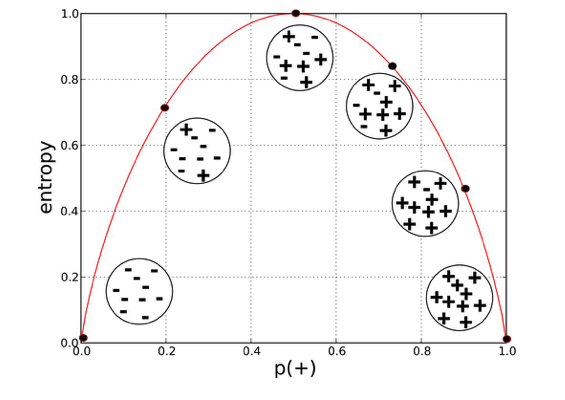
\includegraphics[width=8cm]{figures/1174079/2/entropy.png}
    \centering
    \caption{penggambaran entropi}
\end{figure}
\end{enumerate}



\subsection{Praktek}
Tugas anda adalah, dataset ganti menggunakan student-mat.csv dan mengganti semua nama variabel dari kode di bawah ini dengan nama-nama makanan (NPM mod 3=0), kota (NPM mod 3=1), buah (NPM mod 3=2),
\lstinputlisting[firstline=8, lastline=9]{src/1174079/2/1174079.py} 

\subsubsection{Praktek No. 1}
\hfill\\
\lstinputlisting[firstline=13, lastline=15]{src/1174079/2/1174079.py} 
load library panda sebagai pd kemudian buat variable bernama apel yang diisi dengan function readcsv dari library pd(panda) dan definisikan file yang dimaksud dengan separator titik koma, kemudian perintah len akan mengukur panjang data dari variable apel

\subsubsection{Praktek No. 2}
\hfill\\
\lstinputlisting[firstline=19, lastline=21]{src/1174079/2/1174079.py} 
menentukan pass/fail nya data melalui parameter G1+G2+G3. = 30. kemudian pada variabel mochi dideklarasikan jika baris dengan ut

\subsubsection{Praktek No. 3}
\hfill\\
\lstinputlisting[firstline=25, lastline=26]{src/1174079/2/1174079.py} 
One hot encoding merupakan suatu proses yang digunakan untuk mengkonversi data yang bisa dikelompokkan menjadi bentuk yang bisa di sediakan untuk algoritma machine learning membacanya secara lebih mudah.

\subsubsection{Praktek No. 4}
\hfill\\
\lstinputlisting[firstline=29, lastline=40]{src/1174079/2/1174079.py} 
Variable yang ada diisi dengan data sample yang kemudian dihitung keakuratannya pada bagian printf dengan rumus seperti digambar

\subsubsection{Praktek No. 5}
\hfill\\
\lstinputlisting[firstline=42, lastline=44]{src/1174079/2/1174079.py} 
Import library class tree dari library sklearn kemudian variable mangga diisi dengan function DecisionTreeClassifier dari class tree dengan parameter criteria sebagai entrophy dan maxdepth nya 5 kali, kemudian variable mangga diisi dengan function fit yang akan menghitung data yang ada di parameter dengan metode yang sudah didefinisikan seperti di gambar

\subsubsection{Praktek No. 6}
\hfill\\
\lstinputlisting[firstline=47, lastline=50]{src/1174079/2/1174079.py} 
Graphviz adalah library yang digunakan untuk visualiasasi data, kode kode pada bagian ini kurang lebih hanya untuk visualiasi data berdasarkan data dan aturan dari apa yang telah didefinisikan di variable pir, kemudian pada variable avokado dia memanggil function source untuk meminta sumber data dan settingnya, dan akhirnya ditampilkan

\subsubsection{Praktek No. 7}
\hfill\\
\lstinputlisting[firstline=53, lastline=54]{src/1174079/2/1174079.py} 
tree.export graphviz digunakan untuk membuat  graphic, student-performance dot adalah nama output filenya dan sisanya yaitu parameter yang optional yang digunakan untuk apakah anda ingin menampilkan seluruh data yang ada pada node atau hanya beberapa node saja yang ditampilkan, seperti itu.

\subsubsection{Praktek No. 8}
\hfill\\
\lstinputlisting[firstline=56, lastline=57]{src/1174079/2/1174079.py} 
Score akan membandingkan parameter pertama sebagai hasil yang diinginkan dan parameter kedua sebagai pembanding yang nantinya akan dikalkulasi tingkat kemiripannya dalam bentuk persen

\subsubsection{Praktek No. 9}
\hfill\\
\lstinputlisting[firstline=59, lastline=62]{src/1174079/2/1174079.py} 
Script ini akan akan mecoba untuk mengevaluasi data dengan metode cross validation . Dimana variabel anggur yang  diisi  dengan cross valscore yang merupakan fungsi dari class yang kita import. Kemudian akan memperlihatkan score rata rata dan juga nilai deviasinya

\subsubsection{Praktek No. 10}
\hfill\\
\lstinputlisting[firstline=65, lastline=68]{src/1174079/2/1174079.py} 
script ini berisi tentang perulangan terlebih dahulu yang akan diisi parameternya sebagai 1,20 yang berarti akan diulang perintahnya sebanyak 19 kali, kemudian variable mangga berisi fungsi DecisionTreeClassifier dengan kriteria entropy dengan max-depth yang artinya jumlah fold sebanyak nilai dari variable belimbing, di variable anggur diisi dengan fungsi crossvalscore yang menerima parameter mangga sebagai pengaturan tree, dan apelatt serta apelpass sebagai data dan cv=5 sebagai jumlah foldnya

\subsubsection{Praktek No. 11}
\hfill\\
\lstinputlisting[firstline=71, lastline=80]{src/1174079/2/1174079.py} 
Variable stroberi diisi dengan np yang berarti library numpy lalu memanggil function empty dengan nilai 19,3 dengan tipe data float, lalu ada variable jeruk yang diisi 0, setelah itu ada perulangan belimbing yang diulang sebanyak 19 kali, kemudian ada variable mangga yang diisi function DecisionTreeClassifier dengan settingnya yang sudah dijelaskan sebelumnya, lanjut kebagian variable anggur yang kurang lebih sama seperti penejalasan di nomor 10, kemudian variable stroberi akan mengakses arranya pada bagian yang didefinisikan oleh variable jeruk dan juga 0 yang datanya akan diganti oleh data dari variable belimbing, kemudian variable stroberi akan mengakses bagian yang didefinisikan oleh jeruk, dan 1 yang datanya akan diisi dengan nilai rata rata dari variable anggur, lanjut stroberi akan mengakses array pada bagian yang didefinisikan oleh variable jeruk dan 2 yang akan diisi dengan nilai deviasi dari variable anggur dikali dua, kemudian variable jeruk ditambah 1 lalu menampilkan data stroberi

\subsubsection{Praktek No. 12}
\hfill\\
\lstinputlisting[firstline=83, lastline=86]{src/1174079/2/1174079.py} 
Load library pyplot dari matplotlib sebagai plt, dan buat variable manggis serta pisang yang diisi funtion subplot dari pyplot, kemudian variable pisang memanggil function error bar yang diisi data seperti yang didefnisikan di gambar lalu menampilkannya
\subsection{Penanganan Error}
\subsubsection{Error}
No Module Named Graphviz
\hfill\\

Solusi: 
Pastikan library graphviz terinstall, jika belum buka anaconda prompt kemudian ketika conda install python-graphviz untuk menginstall

\subsection{Bukti Tidak Plagiat}
\begin{figure}[H]
	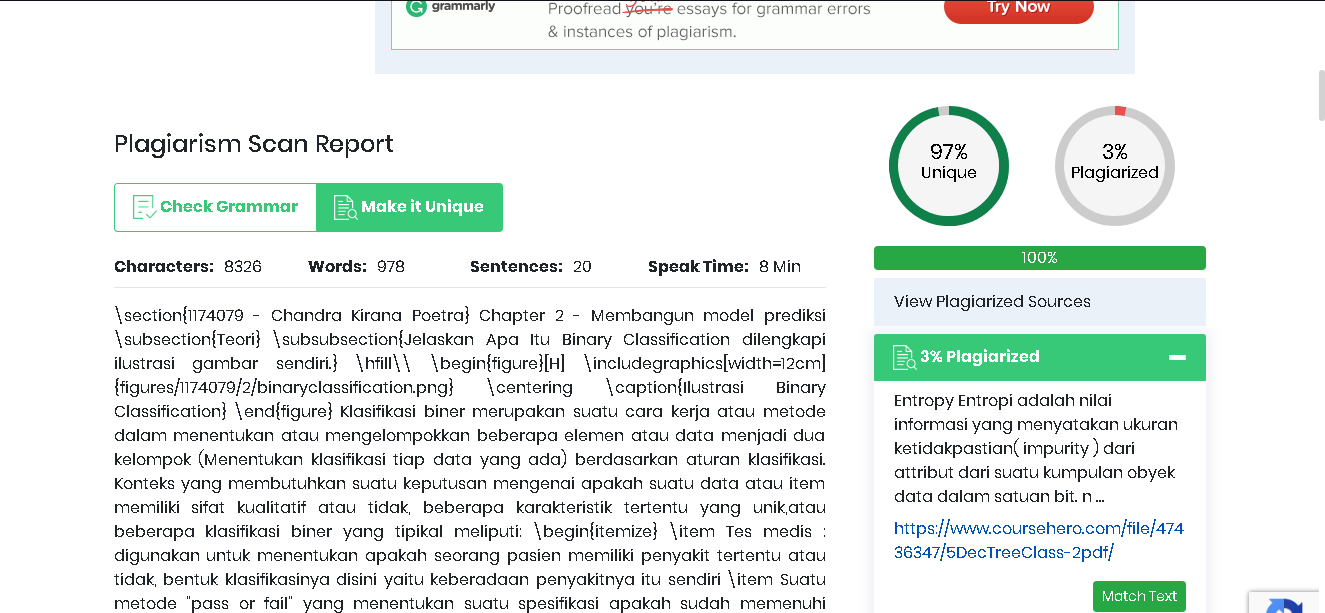
\includegraphics[width=4cm]{figures/1174079/2/plagiarsm.PNG}
	\centering
	\caption{Plagiarism}
\end{figure}

\subsection{Link Video Youtube}
https://youtu.be/9fuSYsqxuVg	
